\documentclass[12pt]{article}

\usepackage[english]{babel}
\usepackage[utf8]{inputenc}
\usepackage{amsthm}
\usepackage{amsmath,amssymb}
\usepackage{parskip}
\usepackage[final]{graphicx}
\usepackage{subcaption}
\usepackage[normalem]{ulem}
\usepackage{titling}
\usepackage[shortlabels]{enumitem}
\usepackage{multirow}
\usepackage{dsfont}
\usepackage{pdfpages}
\usepackage{tikz}
\usepackage{xcolor}
\usepackage{textcomp}
\usepackage{listings}
\usepackage{xparse}
\usepackage{mathtools}
\usepackage{qtree}
\usepackage{wrapfig}
\usepackage[ruled,vlined,linesnumbered]{algorithm2e}
\usepackage{color,soul}

\newcommand\mycommfont[1]{\footnotesize\ttfamily\textcolor{blue}{#1}}
\SetCommentSty{mycommfont}

%% Margins
\usepackage[top=2.5cm, left=3cm, right=3cm, bottom=4.0cm]{geometry}
%% Colour table cells
%% allow code segment, from Overleaf
%%New colors defined below
\definecolor{codegreen}{rgb}{0,0.6,0}
\definecolor{codegray}{rgb}{0.4,0.4,0.4}
\definecolor{codepurple}{rgb}{0.58,0,0.82}
\definecolor{backcolour}{rgb}{0.95,0.95,0.92}

\DeclarePairedDelimiter\abs{\lvert}{\rvert}%%
\DeclarePairedDelimiter\norm{\lVert}{\rVert}%%

% inline code
\NewDocumentCommand{\codeword}{v}{%
\texttt{\footnotesize \textcolor{codegray}{#1}}%
}


%%Code listing style named "mystyle"
\lstdefinestyle{mystyle}{
  backgroundcolor=\color{backcolour}, 
  commentstyle=\color{codegreen},
  keywordstyle=\color{magenta},
  numberstyle=\tiny\color{codegray},
  stringstyle=\color{codepurple},
  basicstyle=\ttfamily\footnotesize,
  breakatwhitespace=false,         
  breaklines=true,                 
  captionpos=b,                    
  keepspaces=true,                 
  numbers=left,                    
  numbersep=5pt,                  
  showspaces=false,                
  showstringspaces=false,
  showtabs=false,                  
  tabsize=4
}

%%"mystyle" code listing set
\lstset{style=mystyle}

%% theorem styles
%% with number
\newtheorem{corollary}{\bf Corollary}[section]
\newtheorem{definition}{\bf Definition}[section]
\newtheorem{proposition}{\bf Proposition}[section]
\newtheorem{Axiom}{\bf Axiom}
\newtheorem{theorem}{\bf Theorem}[section]
\newtheorem{lemma}{\bf Lemma}[section]
\newtheorem{example}{\bf Example}[section]
\newtheorem{remark}{\bf Remark}[section]
\newtheorem{Algorithm}{\bf Algorithm}[section]
\newtheorem{property}{\bf Property}[section]
\newtheorem{note}{\bf Note}
%% with out number
\newtheorem*{corollary*}{\bf Corollary}
\newtheorem*{definition*}{\bf Definition}
\newtheorem*{proposition*}{\bf Proposition}
\newtheorem*{Axiom*}{\bf Axiom}
\newtheorem*{theorem*}{\bf Theorem}
\newtheorem*{lemma*}{\bf Lemma}
\newtheorem*{example*}{\bf Example}
\newtheorem*{remark*}{\bf Remark}
\newtheorem*{Algorithm*}{\bf Algorithm}
\newtheorem*{note*}{\bf Note}
\newcommand{\reff}[1]{Figure~\ref{#1}}
\newcommand{\reftb}[1]{Table~\ref{#1}}

\newcommand\round[1]{\left[#1\right]}

%% mathbb and mathcal often used letters
\newcommand{\Z}{\mathbb{Z}}
\newcommand{\N}{\mathbb{N}}
\newcommand{\Q}{\mathbb{Q}}
\newcommand{\R}{\mathbb{R}}
\newcommand{\C}{\mathcal{C}}
\newcommand{\I}{\mathbb{I}}
\newcommand{\1}{\mathds{1}}
\newcommand{\F}{\mathbb{F}}
\newcommand{\Fp}{\F_{p}}

\newcommand{\<}{\langle}
\renewcommand{\>}{\rangle}

\renewcommand{\hl}[1]{\colorbox{yellow}{#1}}

\newenvironment{solution}{\par\textit{Sol.}}{\hfill $\blacksquare$}
\newcommand{\series}[1][n]{\sum_{#1=1}^{\infty}}
\newcommand{\limil}{\lim\limits}
\newcommand{\inflim}[1][n]{\limil_{#1\rightarrow\infty}}
\newcommand{\sumil}{\sum\limits}
\newcommand{\otherwise}{\text{otherwise}}

\newcommand{\ua}{\uparrow}
\newcommand{\la}{\leftarrow}
\newcommand{\da}{\nwarrow}


%% Get larger line spacing in table
\newcommand{\tablespace}{\\[1.25mm]}
\newcommand\Tstrut{\rule{0pt}{2.6ex}}         %% = `top' strut
\newcommand\tstrut{\rule{0pt}{2.0ex}}         %% = `top' strut
\newcommand\Bstrut{\rule[-0.9ex]{0pt}{0pt}}   %% = `bottom' strut

%% Swap the definition of \abs* and \norm*, so that \abs
%% and \norm resizes the size of the brackets, and the 
%% starred version does not.
\makeatletter
\let\oldabs\abs
\def\abs{\@ifstar{\oldabs}{\oldabs*}}
%%
\let\oldnorm\norm
\def\norm{\@ifstar{\oldnorm}{\oldnorm*}}
\makeatother


\setlength{\droptitle}{-5em}   %% This is your set screw
%% Begin body of paper here

\title{ECS 170: Learning to Play Pong}
\author{Ethan He}
\date{\vspace{-1cm}}

\begin{document}

\maketitle

\section{Problem Representation}

\begin{enumerate}
    \item Since we are using a neural network to replace the Q-table,
        it is easier to use image as state input.
        As it did in the \codeword{QLeaner} class:
\begin{lstlisting}[language=Python]
self.features = nn.Sequential(
    nn.Conv2d(self.input_shape[0], 32, kernel_size=8, stride=4),
    nn.ReLU(),
    nn.Conv2d(32, 64, kernel_size=4, stride=2),
    nn.ReLU(),
    nn.Conv2d(64, 64, kernel_size=3, stride=1),
    nn.ReLU()
)

self.fc = nn.Sequential(
    nn.Linear(self.feature_size(), 512),
    nn.ReLU(),
    nn.Linear(512, self.num_actions)
)
\end{lstlisting}
        % I think it is better to use the hardware ram as array.
        % It might be easier for the agent to learn since the neural network
        % uses array as input and gives array as output.
        % Also image is also stored as matrix of pixels in ram,
        % so eventually the data will be in array form.

    \item The purpose of the neural network in Q-Learning is to replace the lookuo table.
        In such way, we can train a network for each action,
        where we use state as input to the netword and get $\widehat{Q}$ as output.

    \item $\epsilon$ is the identifier for choosing an action.
        We generate a random number,
        if it is greater then $\epsilon$,
        we do exploitation, so choose the best known action that the $Q$ learner tell us;
        otherwise, we do exploration, then do random action.

    \item See function \codeword{act} of \codeword{dpn.py}.
\end{enumerate}



\section{Making a Q-Learner Learn}

The loss function is the square error formula.
In the function, we get the current environment,
where \codeword{batch_size} controls the sample size we fetch from \codeword{replay_buffer} (tensor).
And from the random samples, we find the source to calculate the square error.
The parameter \codeword{gamma}$\gamma$ is to control the Q-learner's behavior:
as $\gamma$ get closer to 1,
future rewards are given greater emphasis relative to the immediate rewards.

\begin{lstlisting}[language=Python]
q_val = torch.gather(model(state.squeeze(1)), 1, action.unsqueeze(1)).squeeze(1) # y_i
q_val_target = target_model(next_state.squeeze(1)).max(1)[0]
expectations = reward + gamma * q_val_target * (1 - done) 
loss = (q_val - Variable(expectations.data)).pow(2).mean()
\end{lstlisting}


\section{Extend the Deep Q-Learner}

See program \codeword{dqn.py}.
\begin{lstlisting}[language=Python]
def sample(self, batch_size):
    # Randomly sampling data with specific batch size from the buffer
    state, action, reward, next_state, done = zip(*random.sample(self.buffer, batch_size))

    state = Variable(torch.FloatTensor(np.float32(state)))
    next_state = Variable(torch.FloatTensor(np.float32(next_state)))

    return state, action, reward, next_state, done
\end{lstlisting}


\section{Learning to Play Pong}

\begin{enumerate}
    \item See program \codeword{run_dqn_pong.py} around line 90.

\begin{lstlisting}[language=Python]
torch.save(model.state_dict(), model_file)
\end{lstlisting}

    \item Use the \codeword{np.savetxt()} function to 
        save \codeword{losses} and \codeword{all_rewards}
        in \codeword{.csv} files for use inquestion 4.

\begin{lstlisting}[language=Python]
np.savetxt("rewards.csv", all_rewards, delimiter=",")
np.savetxt("losses.csv", losses, delimiter=",")
\end{lstlisting}


    \item Use command \codeword{python3 run_dqn_pong.py} to train the model.
    \item Plots.
    
    \begin{figure}[h]
		\subfloat[Rewards]{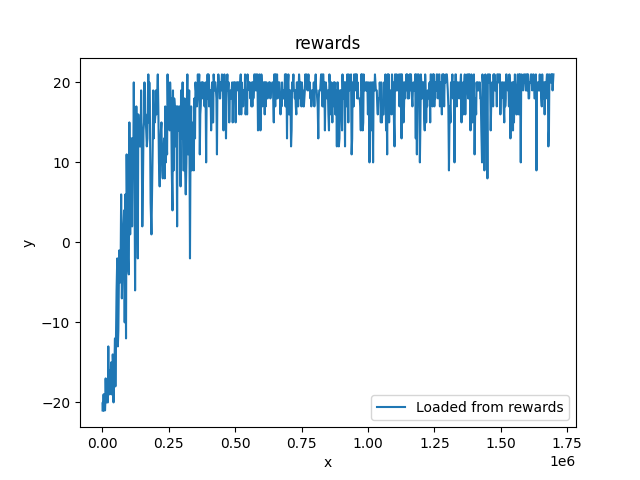
\includegraphics[width = 3in]{./rewards.png}} 
		\subfloat[Losses]{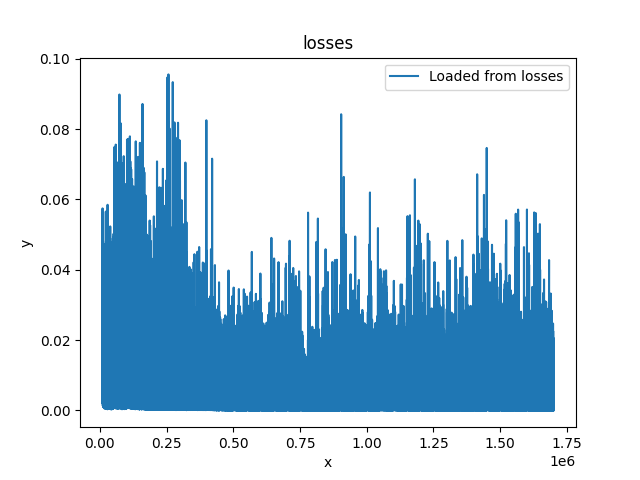
\includegraphics[width = 3in]{./losses.png}}
    \end{figure}

\end{enumerate}


\newpage
\section{Bonus}


\end{document}
